% 20200713
\documentclass[../thesis.tex]{subfiles} %% use packages & commands as this main file
\begin{document}
\section{Methodology}

\subsection{The model}

Our system was a set of ordinary differential equations (ODE).  It contained two biological components (i.e. \phy\ and \bac) and three state variables of densities (i.e. organic carbon $C$, \phy\ biomass $P$ and bacterial biomass $B$) under a standardised temperature range of \temp.  Both biological components received carbon from different sources but performed the same functions (Fig.\ref{f:model}). \Phy\ photosynthesized carbon dioxide from the atmosphere (an unlimited source) and \bac\ consumed carbon from $C$ pool.  Both \phy\ and \bac\ had three ways to allocate carbon: respiration, leakage and biomass incorporation. Some biomass from each component died and became carbon in the $C$ pool.  Organic carbon in the environment could either be consumed by \bac\ or harvested.  Four major assumptions were upheld: 1. environmental conditions was always spatially homogeneous; 2. unlimited nutrient, which was achievable through using sewage as fertilisers \autocite{markou2014microalgal}; 3. high carbon density would not block light; and 4. \bac\ had no preference on any carbon types in the $C$ pool.  In short, living space for \phy\ was the only limiting factor.

Rate of density change of state variables (grams of carbon per metre cube per day, \dxdt) were the subjects in our equations.  The equations were composed of three state variables of densities, two sets of four biological parameters (one set for $P$ and another set for $B$) and one harvest rate parameter (Eq.\ref{eq:PBH}).

\begin{equation}\left\{\begin{array}{rl}
    C'(t) &= \ePR(1-\eP)\cdot\gP\cdot P +\aP\cdot P^2 +(\eBR(1-\eB)-1)\cdot\gB\cdot C\cdot B +\mB\cdot B -xC\\
    P'(t) &= \ePR\cdot\eP\cdot\gP\cdot P -\aP\cdot P^2\\
    B'(t) &= \eBR\cdot\eB\cdot\gB\cdot C\cdot B -\mB\cdot B
\end{array}\right.\label{eq:PBH}\end{equation}

In Eq.\ref{eq:PBH}, $C'(t)$, $P'(t)$ and $B'(t)$ were the rates of density change (\dxdt).  $\ePR$ was the fraction of non-respired carbon for $P$, $\eP$ was the fraction of carbon incorporated as $P$ biomass, $\eBR$ was the fraction of non-respired carbon for $B$ and $\eB$ was the fraction of carbon incorporated as $B$ biomass.  These four were ``fraction parameters”.  $\gP$ was the growth rate of $P$ (\dayU), $\aP$ was the intraspecific interference of $P$ (\denI), $\gB$ was the resource clearance rate of $B$  (\denI) and $\mB$ was the death rate of $B$ (\dayU).  These four were ``rate parameters”.  $x$ was the harvest rate (\dayU), which was the speed of carbon removal from $C$ pool.

\begin{figure}[H]
    \centering
    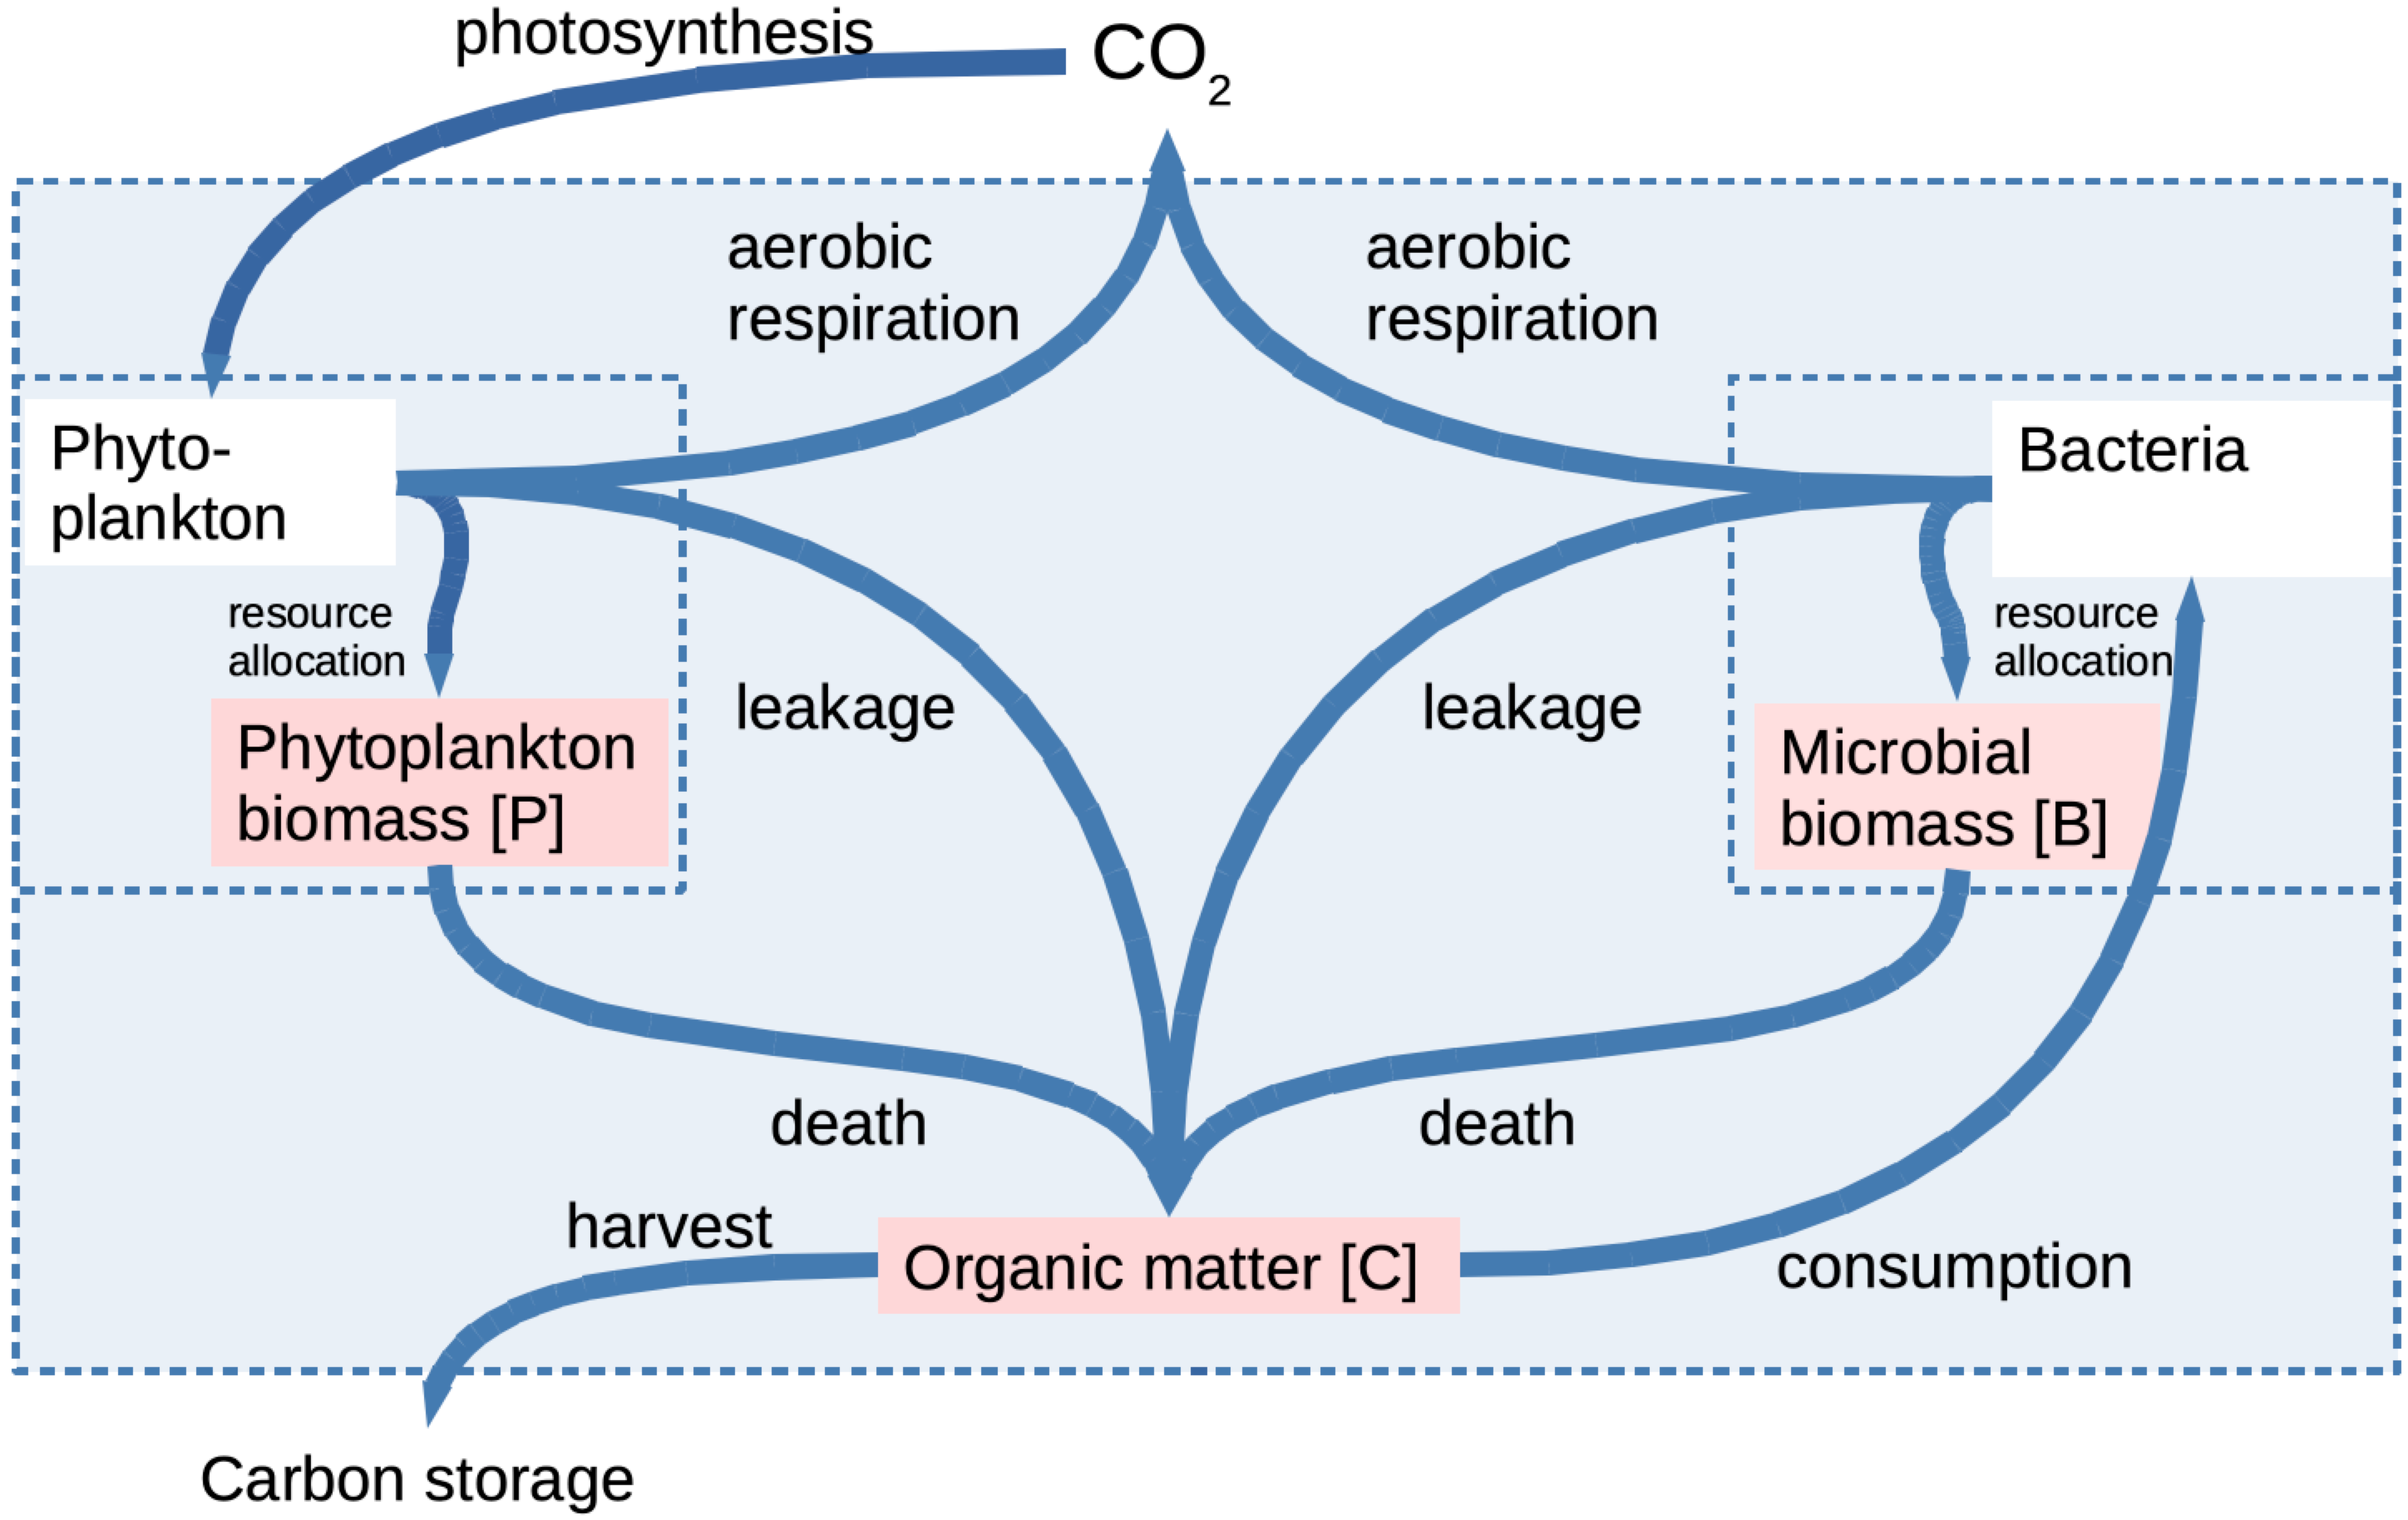
\includegraphics[width=.8\linewidth]{media/model.png}
    \caption[Model visualization]{The theoretical coexistence open system of \phy\ and \bac.  The dashed box was the defined boundary allowed matter exchange.  Blue arrows were the directions of carbon flow with text description above it.  Pink boxes were the carbon pools (i.e. state variables).  White boxes were biochemical processes in indicated organisms.  These processes diverged carbon from source to different carbon pools.}
    \label{f:model}
\end{figure}

Eq.\ref{eq:PBH} was the \pbs\ with continuous harvest (\PBH).  It had three alternatives:

Continuous harvest \phy-only system (\PoH);
\begin{equation}\left\{\begin{array}{rl}
    C'(t) &= \ePR(1-\eP)\cdot\gP\cdot P +\aP\cdot P^2 -xC\\
    P'(t) &= \ePR\cdot\eP\cdot\gP\cdot P -\aP\cdot P^2
\end{array}\right.\label{eq:PoH}\end{equation}

Destructive harvest \pbs\ (\PBN); and
\begin{equation}\left\{\begin{array}{rl}
    C'(t) &= \ePR(1-\eP)\cdot\gP\cdot P +\aP\cdot P^2 +(\eBR(1-\eB)-1)\cdot\gB\cdot C\cdot B +\mB\cdot B\\
    P'(t) &= \ePR\cdot\eP\cdot\gP\cdot P -\aP\cdot P^2\\
    B'(t) &= \eBR\cdot\eB\cdot\gB\cdot C\cdot B -\mB\cdot B
\end{array}\right.\label{eq:PBN}\end{equation}

Destructive harvest \phy-only system (\PoN).
\begin{equation}\left\{\begin{array}{rl}
    C'(t) &= \ePR(1-\eP)\cdot\gP\cdot P +\aP\cdot P^2\\
    P'(t) &= \ePR\cdot\eP\cdot\gP\cdot P -\aP\cdot P^2
\end{array}\right.\label{eq:PoN}\end{equation}

Six algebraic stable system states were found by symbolic solving using SymPy (v1.5.1) in python3 (v3.7.3) (Table \ref{t:eqm}).  Equilibria 3 \& 4 were the only biologically-meaningful defined stable positions.  Defined solutions only contained parameters (not equilibria 5 \& 6) and biologically-meaningful solutions were non-negative densities across all possible state variables (not equilibrium 2) under respective systems.  Hence equilibrium 3 \& 4 represented \PoH\ and \PBH\ respectively; equilibrium 1 was an alternative stable position for both systems.

\begin{table}[H]
    \centering
    \caption[Model equilibria]{Equilibria from the four variations of the proposed model (Eq.\ref{eq:PBH})}
    \begin{tabular}{cl|ccc}\hline
        equilibrium & scenario & $C$ & $P$ & $B$ (\PBH\ \& \PBN\ only) \\\hline
        1 & \PBH, \PoH & 0 & 0 & 0 \\
        2 & \PBH & $\dfrac{\mB}{\eBR\eB\gB}$ & 0 & $\dfrac{-x}{\gB(1-\eBR)}$ \\
        3 & \PBH, \PoH & $\dfrac{\eP(\ePR\gP)^2}{\aP x}$ & $\dfrac{\ePR\eP\gP}{\aP}$ & 0 \\
        4 & \PBH & $\dfrac{\mB}{\eBR\eB\gB}$ & $\dfrac{\ePR\eP\gP}{\aP}$ & $\dfrac{(\ePR\gP)^2\eBR\eB\gB-\aP\mB x}{(1-\eBR)\aP\gB\mB}$ \\
        5 & \PBN & C & 0 & 0 \\
        6 & \PoN & - & P & - \\\hline
    \end{tabular}
    \label{t:eqm}
\end{table}

\subsection{Parameter space}
Data was deficient for half of our defined parameters.  Hence the widest percentage range in respective parameter groups was inferred as the logical range for these data-deficient parameters.  From the defined ranges (Table \ref{t:ranges}), 11 evenly-spaced sample values was selected to form the parameter space for the model.  Method of determining each biological parameter range was in the appendix.

\begin{table}[H]
    \centering
    \caption[Algebra variables]{Biological variables and corresponding ranges framing the parameter space}
    \begin{tabular}{cclll}\hline
        variable & unit & description & min & max \\\hline
        $N'(t)$ & \dxdt & rate of change of respective carbon pool {\tiny($N=C,P,B$)} & - & - \\
        $N$ & \den & carbon density for respective pool {\tiny($N=C,P,B$)} & - & - \\
        $\ePR$ & - & non-respired carbon fraction for $P$ & 0.08 & 0.87 \\
        $\eP$ & - & assimilated carbon fraction for $P$ & 0.40 & 1.00 \\
        $\gP$ & \dayU & growth rate of $P$ & 0.03 & 3.17 \\
        $\aP$ & \denI & intraspecific interference of $P$ & 0.02 & 1.52 \\
        $\eBR$ & - & non-respired carbon fraction for $B$ & 0.13 & 1.00 \\
        $\eB$ & - & assimilated carbon fraction for $B$ & 0.07 & 0.82 \\
        $\gB$ & \denI & clearance rate of $B$ & 0.10 & 3.50 \\
        $\mB$ & \dayU & death rate of $B$ & 0.01 & 0.63 \\
    \hline\end{tabular}
    \label{t:ranges}
\end{table}

\subsection{Scenario sampling}
500 unique biological parameter combinations were randomly selected via a uniform prior with seed number ``20192020" in R (v4.0.2).  This Latin Hypercube Sampling (LHS) method was to ensure the widest parameter space covered with a limited sample size.  Each set of combinations were scanned by 200 evenly-spaced harvest rates (for continuous harvest systems, $x$) ranged from 1 to 19901 \dayU.  Harvest intervals (for destructive harvest systems, $T$, unit: day) was defined as

\begin{equation}
    T = x-1
    \label{eq:TvsX}
\end{equation}

\subsection{Model experiment}
System carbon content in continuous harvest systems was analytically calculated by C-lang (compiler gcc v7.5.0). Yield in \PoH\ was independent from harvest rates because yield was defined as
\begin{equation}
    \text{yield} = x\cdot C
    \label{eq:yield}
\end{equation}

Destructive harvest systems ($x=0$) were integrated by python3 (v3.7.3) SciPy (v1.2.3) ``odeint" function.  Initial densities for \PBN\ and \PoN\ were $C=P=B=1$ and $C=P=1$, $B=0$ \den\ respectively.  Daily yield for destructive harvest systems was defined as
\begin{equation}
    \text{average yield} = \dfrac{[\text{total carbon}]|_{T}-[\text{total carbon}]|_{T=0}}{T}
    \label{eq:avgYd}
\end{equation}

1.1 million ($11\times500\times200$) samples were collected for each system.  We also integrated destructive systems in a log-spaced time ($T$ = 0-100) to observe the system behaviour before stability.

\subsection{Carbon yield analysis}
Feasible/Defined solutions were extracted in two ways for distribution comparisons following the above definition.  Unfeasible solutions were set zero for an overview and set as invalid for observing yield distributions within feasibility limits.  Pairwise Wilcox signed rank tests (R v4.0.2; with bonferroni adjustment and no paired situations) tested significance between system sets with harvest interval/rate contained maximum yield (n=5500) for unfeasible solutions set zero.  Early destructive systems development were plotted on log-spaced time.  Median yield was plotted against the range of harvest intervals/rates.  Effect of \bac\ was compared within each harvest mode on selected harvest intervals/rates.  Effect of biological parameters were deduced through log-yield distributions across each parameter.

\end{document}